\section{Optimisation in Deep Gated Networks}\label{sec:opt}
We study two gating regimes in the paper. The first one is the frozen gating regime which applies for DGNs of the form $\N(\G_{\dagger};\Theta_t)$, which are studied in this section. The second one is the dynamic gating regime which applies for DGNs of the forms $\N(\Tg_t,\beta;\Tw_t)$, $\N(\Theta_t,\beta;\Theta_t)$ and $\N(\Theta_t,\infty;\Theta_t)$, which are dealt with in the next section.

As metioned before $\G_t$ and hence $A_t(\cdot,\cdot)$ specify the manner in which DGNs finds two inputs similar to each other. By studying $\N(\G_{\dagger};\Theta_t)$  DGNs, we first keep the gates constant (recall that $\G_{\dagger}$ means $\G_t=\G_0,\forall t\geq 0$), and understand the effect of SGD on the path strengths. To this end, we study the following types of $\N(\G_{\dagger};\Theta_t)$ DGNs:

%In this section, we consider $\N(\G_{\dagger}, \Theta_t)$ DGNs. In particular, we consider the following interesting cases:

$1.$ \emph{Deep Linear Networks (DLN):} These are $\N(1_{\dagger}; \Theta_t)$, where all the gating values are $1$. Here, we do not have any control over how the paths are formed, since all the paths are \emph{always on}.

$2.$ \emph{Fixed Random Gating (DGN-FRG): } Note that $\G_0$ contains $n\times (d-1)\times w$ gating values, corresponding to the $n$ input examples, $(d-1)$ layers and $w$ nodes in each layer. $\G_0\in \{0,1\}^{n\times (d-1)\times w}$, where each gating values is chosen to be $0$ or $1$ with probabilities $1-p$ and $p$ respectively. We denote these DGNs by $\N(Ber(p)_{\dagger};\Theta_t)$. Here, we have full control over the gating/activation level of the paths. These networks are restricted solely towards understanding questions related to optimisation. Generalisation is irrelevant for DGN-FRG networks because this no natural means to extend the random gate generation for unseen inputs, or in other words, it is not clear what gating values are to be used for unseen inputs.

$3.$ \emph{Gated Linear Units (GaLU):} Here we consider DGNs of the form $\N(\Tg_{\dagger},\infty;\Tw_t)$, i.e., the gating network contains ReLU gates whose values are copied and used in the weight network which is trained. Here, we do not have full freedom over gating/activation as it is with DGN-FRG networks. However, these networks can generalise in a natural way.


Since the gates are fixed $\Psi^a_t=0,\forall t\geq 0$, and only the path strengths are sensitive to $\Theta_t$. The neural tangent features of the path strengths (NTFPS) in \Cref{def:ntfps} as follows:

\begin{definition}\label{def:ntfps}[NTFPS]
\begin{align}
\varphi^w_{t,p}\stackrel{def}{=}\left(\frac{\partial w_{t}(p)}{\partial \theta(m)},m\in[d_{net}]\right)\in \R^{d_{net}},
\end{align}
\end{definition}
%Let $p\rsa\theta(m)$ be a short hand to denote the fact that path $p$ pass through weight $\theta(m)$.
\begin{remark}
Let $\theta(m)$ belong to layer $l'\in [d-1]$, then 
\begin{align*}
\varphi^w_{t,p}(m)&=\underset{l\neq l'}{\underset{l=1}{\overset{d}{\Pi}}} \Theta_t(l,p(l-1),p(l)), \forall p\rsa\theta(m)\\
&=0, \forall p\bcancel{\rsa}\theta(m)
\end{align*}
\end{remark}

\begin{remark}\label{rm:basicgram}
\begin{align*}
{K^w_t(s,s')}=\sum_{i=1}^{d_{in}} x(i,s)x(i,s') \lambda^{s,s'}_t(i),
\end{align*}
where
\begin{align*}
&\lambda^{s,s'}_t(i)\stackrel{def}=\underset{p_1,p_2\rsa\theta(m),i}{\sum_{p_1,p_2\in P:}}  \varphi_{t,p_1}(m)A(s,p_1)  \varphi_{t,p_2}(m) A(s',p_2)
\end{align*}

%\begin{align*}
%&{K^w_t(s,s')}=\sum_{m=1}^{d_{net}} \Bigg(\underset{p_1,p_2\rsa\theta(m)}{\sum_{p_1,p_2\in P:}} x(p_1(0),s) \varphi_{t,p_1}(m) \\
%&A(s,p_1)  x(p_2(0),s') \varphi_{t,p_2}(m) A(s',p_2)\Bigg)\\
%&=\sum_{i=1}^{d_{in}} x(i,s)x(i,s') \lambda_{s,s'}(i)
%\end{align*}
\end{remark}

\begin{assumption}\label{assmp:mainone}
$\G_0$ is statistically independent of $\Theta_0$.
\end{assumption}
\textbf{Decoupling of gates and paths:} In a standard DNN with ReLU activations, the activations and weights are not statistically independent because conditioned on the fact that a ReLU is \emph{on}, the incoming edges cannot be simultaneously all $-\sigma$. 
We side step this issue by Assumption~\ref{assmp:main}, wherein, we assume that  gating is statistically independent of the weights $\Theta_0$. 


\begin{assumption}\label{assmp:maintwo}
$\Theta_0\stackrel{iid}\sim Ber(\frac{1}{2})$ over the set $\{-\sigma,+\sigma\}$. 
\end{assumption}
\textbf{Decoupling of paths from one another}, which stands for the fact that the inner product of NTFPS of two different paths is $0$ on expectation. This is captured in Lemma~\ref{lm:pathdot} below.

%\begin{figure}
%\centering
%\includegraphics[scale=0.2]{mickey.png}
%\caption{Shows that the incoming weights of a ReLU gate which are \emph{on} are not symmetrically distributed.}
%\end{figure}
\FloatBarrier
\begin{figure*}[h]
\resizebox{\textwidth}{!}{
\begin{tabular}{cccc}
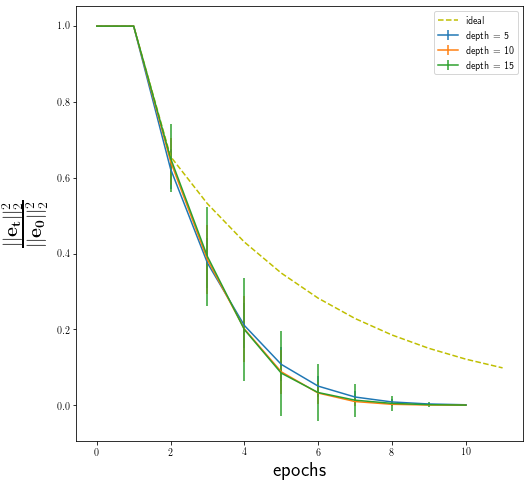
\includegraphics[scale=0.4]{figs/dln.png}
&
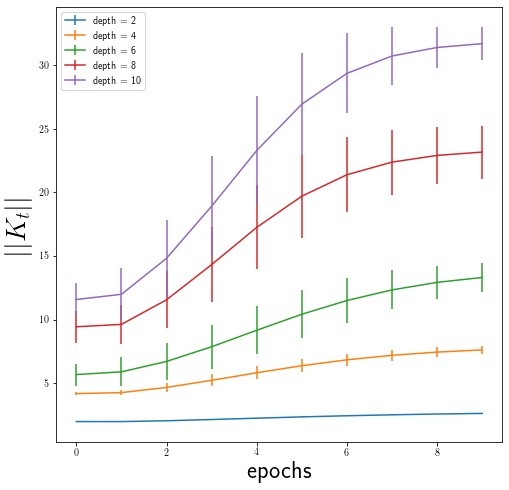
\includegraphics[scale=0.4]{figs/dln-gram.png}
&
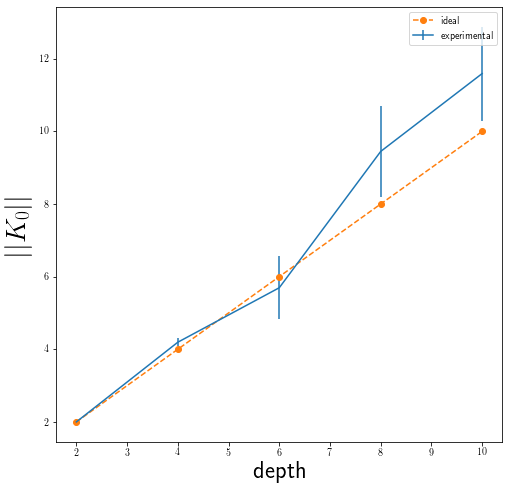
\includegraphics[scale=0.4]{figs/dln-k-vs-d.png}
&
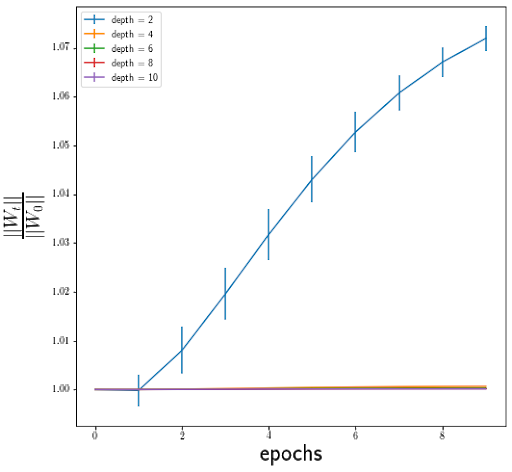
\includegraphics[scale=0.4]{figs/dln-norm.png}
\end{tabular}
}
\caption{Shows plots for deep linear networks.}
\label{fig:dlnplots}

\end{figure*}


\begin{lemma}\label{lm:pathdot}
Let $\theta(m)$ be an arbitrary weight in layer $l'\in [d-1]$, under Assumption~\ref{assmp:init} we have for paths $p,p_1,p_2\rsa\theta(m), p_1\neq p_2$
\begin{align*}
\E{\varphi_{\Tb,p_1}(m)\varphi_{\Tb,p_2}(m)}= &0\\
\E{\varphi_{\Tb,p}(m)\varphi_{\Tb,p}(m)}= &\left(\frac{2\sigma^2}{w}\right)^{d-1}
\end{align*}
\end{lemma}
\begin{proof}
If $\theta$
Note that $\varphi_{\Tb,p}=\underset{l\neq l'}{\underset{l=1}{\overset{d}{\Pi}}} \Tb(l,p(l-1),p(l))$. Hence
\begin{align*}
&\E{\varphi_{\Tb,p_1}(m)\varphi_{\Tb,p_2}(m)}\\
&=\E{\underset{l\neq l'}{\underset{l=1}{\overset{d}{\Pi}}} \Bigg(\Tb(l,p_1(l-1),p_1(l))\Tb(l,p_2(l-1),p_2(l)) \Bigg)}\\
&=\underset{l\neq l'}{\underset{l=1}{\overset{d}{\Pi}}}\E{\Tb(l,p_1(l-1),p_1(l))\Tb(l,p_2(l-1),p_2(l))}
\end{align*}

Since $p_1\neq p_2$, in one of the layers $\tilde{l}\in[d-1],\tilde{l}\neq l'$ they do not pass through the same weight. Using this fact
\begin{align*}
&\E{\varphi_{\Tb,p_1}(m)\varphi_{\Tb,p_2}(m)}\\
&=\left(\underset{l\neq l',\tilde{l}}{\underset{l=1}{\overset{d}{\Pi}}}\E{\Tb(l,p_1(l-1),p_1(l))\Tb(l,p_2(l-1),p_2(l))}\right)\\
&\Bigg(\E{\Tb(\tilde{l},p_1(\tilde{l}-1),p_1(\tilde{l}))}\E{\Tb(\tilde{l},p_2(\tilde{l}-1),p_2(\tilde{l}))}\Bigg)\\
&=0
\end{align*}
\end{proof}


\begin{theorem}\label{th:dgnexp}
Let 
\begin{align*}
\mu^{s,s'}(i)\stackrel{def}=\sum_{m=1}^{d_{net}} \underset{p\rsa\theta(m)}{\sum_{p\in P: p(0)=i}}A(s,p) A(s',p),
\end{align*} then under Assumptions~\ref{assmp:mainone},~\ref{assmp:maintwo} if follows that
 \begin{align*}
 \mathbf{E}_{\Theta_0}\left[\lambda^{s,s'}_0(i)\right]&=\sigma^{2(d-1)}\mu^{s,s'}(i)\\
\mathbf{E}_{\Theta_0}\left[K_0(s,s')\right]&=\sigma^{2(d-1)}\sum_{i=1}^{d_{in}}x(i,s) x(i,s')\mu^{s,s'}(i)\\
Var\left[K_0\right]&\leq 
\end{align*}
\comment{
\begin{align*}
&\mathbf{E}_{\Tb}\left[K_0(s,s')\right]=\sigma^{2(d-1)}\left(\sum_{i=1}^{d_{in}}x(i,s) x(i,s')\right.\\
& \left.  \Bigg(\sum_{m=1}^{d_{net}} \underset{p\rsa\theta(m)}{\sum_{p\in P: p(0)=i}}A(s,p) A(s',p)\Bigg)\right)\\
\end{align*}}

\end{theorem}
\begin{proof}
See Appendix.
\end{proof}
\textbf{Remark:} Note that in the case of gates taking values in $\{0,1\}$, $\mu^{s,s'}(i), i\in [d_{in}], s,s'\in [n]$, is a measure of the sub-networks that start at input node $i$, and are active for both input examples $s,s'$ and pass through the weights $\theta(m), m\in[d_{net}]$. 

\comment{
\subsection{Capturing the activation dynamics}

While in a standard DNN with ReLU activations keep dynamically changing, $\Psi^a_t$ cannot be well defined at the same time because for infinitesimal change the activations do not change. We address this issue by considering a soft-max version of ReLU gate: let $x_in$ and $x_out$ be the input and output of a gate, then the ReLU and soft-max ReLU are given by
\begin{align*}
&\text{ReLU:}\,&x_{out}&=\max\{x_{in},0\}\\
&\text{Soft-Max:}\,&G(x_{out})&=\frac{1+\epsilon}{1+exp(-\beta x_{in})}
\end{align*}
Without the $\epsilon>0$ the soft-max output will be less than $1$, since $A=\Pi _{l=1}^{d-1}G$, the activations can die down with depth. The $1+\epsilon$ ensures that activations do not die down over the depth. Both $\Tb$ and $\Tg$ have the same cardinality given by $d_{net}$.

\begin{definition}
Let $\gamma>0$ be a threshold value, and let $z(i,l)$ denote the input of the node $i$ in layer $l$. We say that the gate to be `transitioning' for input $s$ if
\begin{align}
\left|\frac{\partial G_{\Tg}(s,i,l)}{\partial z(i,l)}\right|>\gamma,
\end{align}
and define a gate to be `flipped' (to $0$ or $1$) otherwise.
\end{definition}
\begin{assumption}\label{assmp:gating}
For any input $s\in [n]$, we assume that a weight $\tg(m)$ affects the gating pattern $G_{\Tg}(\cdot,i_m,l_m)$ at node $i_m$ in layer $l_m$ for some indices $i_m, l_m$ dependent on $m$:
\begin{align*}
\frac{\partial G_{\Tg}(s,i,l')}{\partial \tg(m)}&=0,\forall i\neq i_m\\
\frac{\partial G_{\Tg}(s,i',l)}{\partial \tg(m)}&=0,\forall l\neq l_m
\end{align*}
\end{assumption}


\begin{lemma}
Let $\tg(m)$ be associated with a fixed node $(i_m,l_m)$ as in \Cref{assmp:gating}

i) $\frac{\partial A_{\Tg}(s,p)}{\partial \tg(m)}=0,\forall p \bcancel{\rsa}O(i',l')$.

ii) $\frac{\partial A_{\Tg}(s,p)}{\partial \tg(m)}\approx \frac{\partial G_{\Tg}(s,i,l)}{\tg(m)},\forall p{\rsa}O(i',l')$ and such that all other gates through which $p$ passes are flipped to $1$.

\end{lemma}

}
\comment{

\section{DNN with fixed activations}\label{sec:fixedg}
In this section, we look at three interesting cases of DNN with fixed gating patterns, i.e., gating pattern $G$ does not change with time. These are: \begin{enumerate} \item Deep Linear Networks (DLN). \item Deep Gated Networks with fixed random activation (DGN-FRA).  \item Deep Gated Networks with fixed dependent activations (DGN-FDA). \end{enumerate} 
In all these cases $\Phi^a_t=0$, i.e., the activations are fixed over time, and hence $K_t=K^w_t$, where $K^w_t\stackrel{def}={\Psi_t^w}^\top \Psi_t^w$. 
\begin{lemma}\label{lm:gramflat}
\begin{align*}
&{K^w_t(s,s')}=\sum_{m=1}^{d_{net}} \Bigg(\underset{p_1,p_2\rsa\theta(m)}{\sum_{p_1,p_2\in P:}} x(p_1(0),s) \varphi_{\Tb,p_1}(m) \\
&A(s,p_1)  x(p_2(0),s') \varphi_{\Tb,p_2}(m) A(s',p_2)\Bigg)
\end{align*}
\end{lemma}


}


\subsection{Deep Linear Networks}
In this case, $G(s,l,i)=1,\forall s\in[n],i\in[w],l\in[d-1]$. Note that all the paths are always active irrespective of which input is presented to the DLN. We can define the effective weight that multiplies each of the input dimensions as follows:
\begin{align}
\eta_{t}(i)= \sum_{p\in P: p(0)=i} w_{t}(p), i\in [d_{in}]
\end{align}
Using the above definition of $\eta=(\eta(i),i\in[d_{in}])\in \R^{d_{in}}$. The hidden feature representation can be simplified as follows:
\begin{align}
\hat{y}_t&=\Phi^\top_{x,1_{\dagger}} w_{t}\\
&=x^\top \eta_{t}
\end{align}
Thus it is clear that the DLN does not provide any high dimensional feature representation and the input features are retained as such. All that the depth adds is just a non-linear re-parameterisation of the weights.

Also note that since $A(s,p)=1,\forall p$ it follows that $\lambda^{s,s'}_t(i)=\lambda_t(i),\forall s,s'\in [n]$. Thus the Gram matrix can be reduced to 
\begin{align}
K_t=x^\top \Lambda_t x, 
\end{align}
where $\Lambda_t$ is an $d_{in}\times d_{in}$ diagonal matrix whose diagonal entries are $\lambda_t(i)$.

\comment{

In a similar manner to the hidden feature, the NTF matrix can also be reduced in the DLN using the fact that $A(s,p)=1,\forall s\in [n], p\in P$, as follows:
\begin{align}
\sum_{p\in P} x(p(0),s) \varphi_{\Tb,p} A(s,p) =\sum_{i=1}^{d_{in}} x(i,s)\sum_{p\in P:p(0)=i}  \varphi_{\Tb,p}
\end{align}

which in turns implies that rank of the $d_{net}\times n$ NTK matrix $\Psi_t$ is utmost $d_{in}$, and hence the number of non-zero eigenvalues of $K_t$ is utmost $d_{in}$.

}
\subsubsection{Learning $1$-dimensional value}
We first consider data set with $n=1$, and $d_{in}=1$, i.e., given $x=1\in \R$ and $y\in \R$, we want to learn $\Tb_*$ such that 
\begin{align}
y=x\eta_{\Tb_*},
\end{align}
In this case $K_t\in \R$, and we now look at its properties at initialisation. 
\comment{
\begin{assumption}\label{assmp:init}[Initialisation]
We assume that at initialisation the weights $\Tb$ are chosen iid with weights taking values from the set $\{ -\sigma,\sigma \}$ with equal probability.
\end{assumption}
}
\begin{corollary}\label{th:dln}\hfill\\
$\mathbf{E}_{\Tb}\left[K_0\right]=d(w\sigma^2)^{2(d-1)}$.
\end{corollary}
The proof follows by noting that $A(s,p)=1$ in \Cref{lm:gramflat}, and applying \Cref{lm:pathdot}.  Please look at the Appendix for a detailed.

\textbf{Experiment:} We consider a dataset with $n=1$ and $(x,y)=(1,1)$. We consider $\N(1_{\dagger},\Theta_t)$, for $d_{in}=1$, $w=100$, and $d=5,10,15$. We set $\sigma=\sqrt{\frac{1}{w}}$ and the weights are drawn according to Assumption~\ref{assmp:main}. We set the learning rate to be $\alpha=\frac{0.1}{d}$, and for this setting we expect the error dynamics to be the following:
\begin{align*}
e_{t+1}&=e_t-\frac{0.1}{d}d(w\sigma^2)^{2(d-1)}e_t\\
&=0.9^te_t
\end{align*}
The results are shown in \Cref{fig:dlnplots}. We observe that irrespective of the depth the error dynamics is similar (since $\alpha=\frac{0.1}{d}$ ). However, we observe faster convergence of error to zero since the magnitude of $K_t$ increases with time (see \Cref{fig:dlngrow}).

\begin{figure*}
\resizebox{\textwidth}{!}{
\begin{tabular}{cccc}
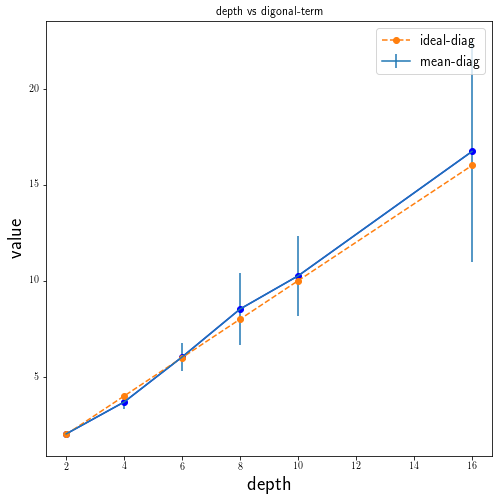
\includegraphics[scale=0.4]{figs/dgn-frg-diag.png}
&
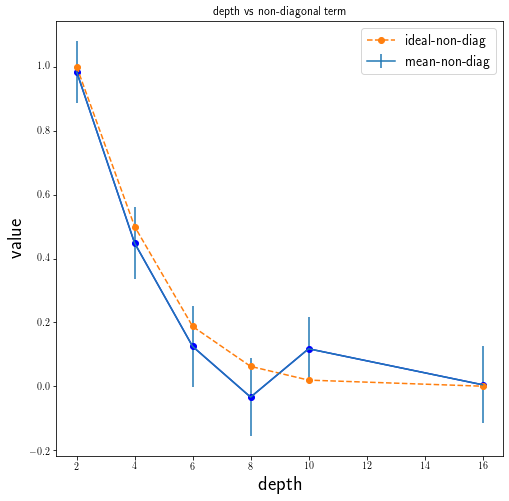
\includegraphics[scale=0.4]{figs/dgn-frg-non-diag.png}
&
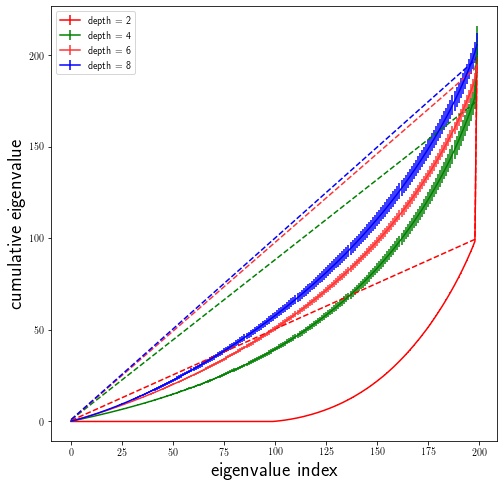
\includegraphics[scale=0.4]{figs/dgn-frg-ecdf-w100.png}
&
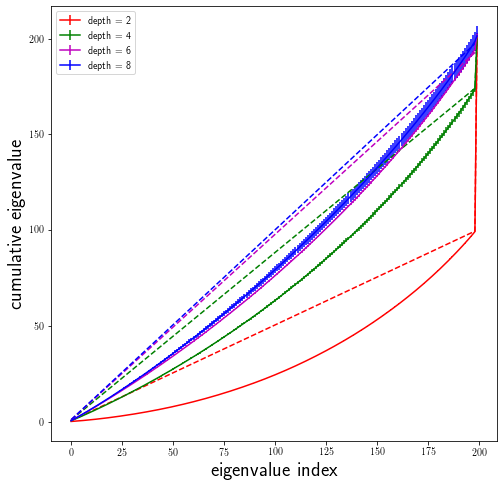
\includegraphics[scale=0.4]{figs/dgn-frg-ecdf-w500.png}
\end{tabular}
}
\caption{Shows the plots for $\N(Ber(p)_{\dagger};\Theta_t)$. The left most and second from left plots respectively show the diagonal and non-diagonal (chosen arbitrary) entries of $K_0$ (for setting $\sigma=\frac{1}{pw}$ averaged over $20$ runs. The first and second from right plots respectively show the e.c.d.f for $w=500$ and $w=100$ respectively. }
\label{fig:dgn-frg}
\end{figure*}

\subsection{Deep Gated Networks with Fixed Random Gating (DGN-FRG)}
In $\N(Ber(p)_{\dagger};\Theta_t)$ DGNs, the sub-network which is active for each input example is random, and the overlap of paths for different inputs will be the same on expectation. This is captured in Lemma~\ref{lm:dgn-fra} below.
\comment{
\textbf{NTK Matrix:} Now we look at the case where $G(s,i,l)\stackrel{iid}\sim Ber(p)$\footnote{$X\sim Ber(p)$ are Bernoulli random variables with $P(X=1)=p$ and $P(X=0)=1-p$.} Note that the activation of a path $A(s,p)$ is different for different inputs: i.e., a given path can either be active or inactive for a given input or alternatively the set of active paths $on(s)=\{p\in P: A(s,p)=1\}$ changes from input to input. In other words, each row of the NTK matrix is formed by a linear combination of the tangent feature of paths that are active i.e., $\Psi_t(\cdot,s)= \sum_{p\in on(s)} x(p(0),s) \varphi_{\Tb,p}$, which differs across inputs, and hence the rank of the $\Psi_t$ matrix (and also the Gram matrix $K_t$) can be utmost $d_{net}$.


\begin{theorem}\label{th:dgn-fra}
 Under \Cref{assmp:init}
\begin{align*}
\text{i)}\, &\mathbf{E}_{\Tb}\left[K_0(s,s')\right]=\sigma^{2(d-1)}\left(\sum_{i=1}^{d_{in}}x(i,s) x(i,s')\right.\\
& \left.  \Bigg(\sum_{m=1}^{d_{net}} \underset{p\rsa\theta(m)}{\sum_{p\in P: p(0)=i}}A(s,p) A(s',p)\Bigg)\right)\\
%\text{ii)}\, &Var_{\Tb}\left[K_0(s,s')^2\right]=O\left(\frac{d_{in}^2d}{w^2} (2p\sigma^2)^{d-1} \right)
\end{align*}
\end{theorem}
The proof of \Cref{th:grambasic} is in the Appendix.

}

\begin{lemma}\label{lm:dgn-fra}
\begin{align*}
\mathbf{E}_{Ber(p)_{\dagger}}\left[\mu^{s}\right]&= d(pw)^{d-1}\\
\mathbf{E}_{Ber(p)_{\dagger}}\left[\mu^{s,s'}\right]&= d(p^2w)^{d-1}
\end{align*}
\end{lemma}
\comment{
\begin{lemma}
\begin{align*}
\E{\sum_{m=d_{in}w+1}^{d_{net}-w} \underset{p\rsa\theta(m)}{\sum_{p\in P: p(0)=i}}A(s,p)A(s,p)}= (d-1)(pw)^{d-1}\\
\E{\sum_{m=d_{in}w+1}^{d_{net}-w} \underset{p\rsa\theta(m)}{\sum_{p\in P: p(0)=i}}A(s,p)A(s',p)}= (d-1)(p^2w)^{d-1},
\end{align*}
where $\E{\cdot}$ is over the randomised assignments of the gating patterns.
\end{lemma}
}
\begin{proof}
Note that since $A$ is a $0/1$ random variable, $A^2=A$. The outer summation is over the weights in the layers $2,\ldots,d-1$, of which only those weights whose input and output gates are active have the inner summation to be non-zero, else the inner summation is $0$. Thus only $(d-1)(pw)^2$ terms survive the outer summation on expectation.The expected number of gates active per layer is $pw$, and hence the expected number of active paths is $d_{in}(pw)^{d-1}$. Tthe expected total number of active paths staring from a given input node $i$ and passing through a weight in layers $2,\ldots,d-1$ is $(pw)^{d-3}$. Putting everything together, we have $(d-1)(pw)^2(pw)^{d-3}=(d-1)(pw)^{d-1}$.

The second expression follows from the fact that for $2$ different inputs $s,s'$ we have the probability term to be $p^2$ instead of $p$.
\end{proof}
\comment{
\begin{figure}[h]
\centering
\includegraphics[scale=0.25]{mickey.png}
\caption{Shows the overlap of paths for two different inputs passing through a given weight $\theta(m)$}
\label{pathoverlap}
\end{figure}
}

\textbf{Deep Information Propagation:} For $\sigma=\sqrt{\frac{1}{pw}}$, the expected Gram matrix divided by the depth $d$ can we written as :
\comment{
\begin{align*}
\frac{\E{K_0}}{d}=\left[\begin{matrix}
\ip{x_1,x_1} &\ip{x_{1},x_s}p^{d-1}&\ldots &\ip{x_1,x_{s'}}p^{d-1} &\ldots\\
\vdots &\ip{x_s,x_s}\quad\quad &\ldots &\ip{x_s,x_{s'}}p^{d-1} &\ldots\\ 
\vdots &\ip{x_{s'},x_s}p^{d-1} &\ldots &\ip{x_{s'},x_{s'}} &\ldots \\
\vdots &\ip{x_{1},x_s}p^{d-1}&\ldots &\ip{x_1,x_{s'}}p^{d-1} &\ip{x_n,x_n} \\
\end{matrix}\right]
\end{align*}
}
\begin{align*}
\frac{\E{K_0}}{d}=\left[\begin{matrix}
\cdot &\ip{x_1,x_s}p^{d-1} &\cdot &\quad\quad\ip{x_1,x_{s'}}p^{d-1} &\cdot\\ 
\cdot &\ip{x_s,x_s}\quad\quad &\cdot &\quad\quad\ip{x_s,x_{s'}}p^{d-1} &\cdot\\ 
\cdot &\ip{x_{s'},x_s}p^{d-1} &\cdot &\ip{x_{s'},x_{s'}} &\cdot \\
\cdot &\ip{x_n,x_s}p^{d-1} &\cdot &\quad\quad\ip{x_n,x_{s'}}p^{d-1} &\cdot\\ 
\end{matrix}\right]
\end{align*}


\comment{
$\bullet$ \textbf{Diagonal Terms of $\E{K_0}$:} Supposing inner double summation can be pulled out in $\E{K_0(s,s)}$ in the right hand side, and replaced by it is expected value, we can surmise that the diagonal term is roughly  $(d-1)(2p\sigma^2)^{d-1}\ip{x(\cdot,s),x(\cdot,s')}$. Now letting $\sigma=1$, and $p=\frac{1}{2}$, we have the diagonal terms to be $(d-1)\ip{x(\cdot,s),x(\cdot,s')}$. 

$\bullet$ \textbf{Cross Terms of $\E{K_0}$:} Supposing inner double summation can be pulled out in $\E{K_0(s,s')}$ in the right hand side, and replaced by it is expected value, we can surmise that the cross terms can be  $(d-1)(2p^2\sigma^2)^{d-1}\ip{x(\cdot,s),x(\cdot,s')}$. Now letting $\sigma=1$, and $p=\frac{1}{2}$, we have the cross terms to be $(d-1)p^d\ip{x(\cdot,s),x(\cdot,s')}$. Thus the input gets \emph{disentangled} and the Gram matrix gets whitened as depth increases.
}


\textbf{Experiments:} Consider the dataset $(x_s,y_s)_{s=1}^n\in \R\times \R$, where $x_s=1,\forall s\in [n]$, and $y_s\sim unif([-1,1])$. The input Gram matrix $x^\top x$ is a $n\times n$ matrix with all entries equal to $1$ and its rank is equal to 1. This is the worst possible case, since all the inputs are identical. However, a fact that saves the day, is that in DGN-FRG, the active sub-network for each input is chosen at random. For this example we have:
\begin{align}\label{eq:mat}
\frac{\E{K_0}}{d}=\left[\begin{matrix}
1 &p^{d-1} &\ldots &p^{d-1} &\ldots\\ 
\ldots &1 &\ldots &p^{d-1} &\ldots\\ 
\ldots &p^{d-1} &\ldots &1 &\ldots \\
\ldots &p^{d-1} &\ldots &p^{d-1} &1\\ 
\end{matrix}\right]
\end{align}
i.e., all the diagonal entries are $1$ and non-diagonal entries are $p^{d-1}$. Now, let $\rho_i\geq 0,i \in [n]$ be the eigenvalues of $\frac{\E{K_0}}{d}$, and let $\rho_{\max}$ and $\rho_{\min}$ be the largest and smallest eigenvalues. From the structure of \eqref{eq:mat}, one can easily show that $\rho_{\max}=1+(n-1)p^{d-1}$ and corresponds to the eigenvector with all entries as $1$, and $\rho_{\min}=(1-p^{d-1})$ repeats $(n-1)$ times, for which corresponds to eigenvectors are given by $\left[0, 0, \ldots, \underbrace{1, -1}_{\text{$i$ and $i+1$}}, 0,0,\ldots, 0\right]^\top \in \R^n$ for $i=1,\ldots,n-1$.


\textbf{Effect of depth $d$:} We first fix arbitray diagonal and non-diagonal entries, and look at their value averaged over $20$ run (see \Cref{fig:dgn-frg}). The actual values (shown in bold) indeed follow the ideal values (as in \eqref{eq:mat})) are shown in the dotted lines. Next, we look at the cumulative eigenvalue, or, e.c.d.f obtained by first sort the eigenvalues in ascending order then looking at their cumulative sum. The ideal behaviour as predicted from theory is that, indices $k\in[n-1]$ indices, the e.c.d.f should increase at a linear rate $k(1-p^{d-1})$, and the difference between the last two indices is $1+(n-1)p^{d-1}$. In \Cref{fig:dgn-frg}, we plot the e.c.d.f for various depths for two different width namely $w=100,500$. Firstly, we while we observe that there is a difference between the actual and ideal curves, we note that the cumulative sum of the first $(n-1)$ values and the maximum eigenvalue does match according to theory. The difference is the cumulative sum in the first $(n-1)$ indices is due to the variance in the entries of the Gram matrix. It can be seen that the effect of variance is less pronounced for $w=500$, in that, the difference between the ideal and actual curves when compared to $w=100$.

\textbf{Effect of $p$} is shown in \Cref{fig:peff}. For $w=100$, we observe that for  the e.c.d.f gets better as the value of $p$ reduces till $p=0.3$, after which it starts degrading. This is due to the fact that the variance gets worse with $\frac{1}p$. It can be seen that for $w=50$ the variance is more and hence the e.c.d.f gets better as we reduce $p$ only till $p=0.4$, after which it starts to degrade.

\FloatBarrier
\begin{figure}[h]
\resizebox{\columnwidth}{!}{
\begin{tabular}{cc}
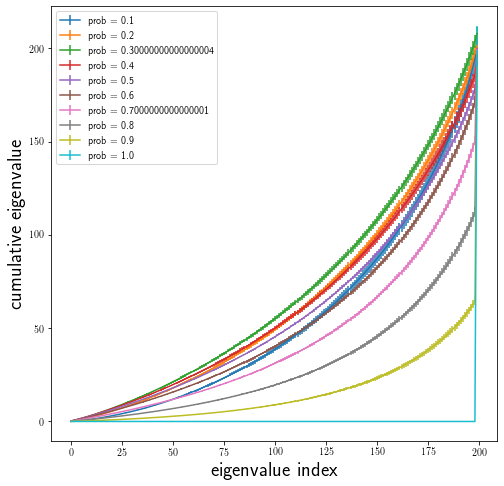
\includegraphics[scale=0.3]{figs/dgn-frg-ecdf-p-w100.png}
&
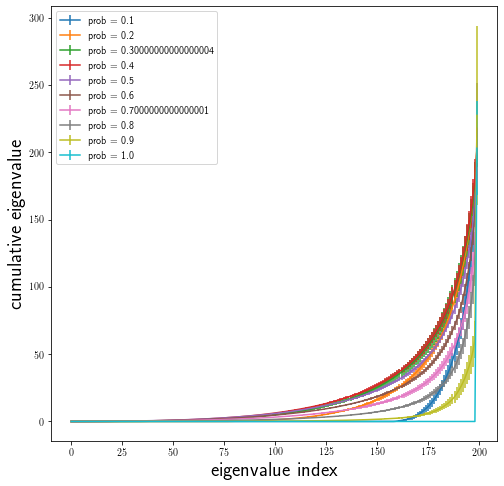
\includegraphics[scale=0.3]{figs/dgn-frg-ecdf-p-w10.png}
\end{tabular}
}
\caption{Shows e.c.d.f for various values of $p$.}
\label{fig:peff}
\end{figure}

\textbf{Convergence} In order to compare how the rate of convergence varies with the depth we set the step-size $\alpha=\frac{0.1}{\rho_{\max}}$. Thus at the start, the maximum eigenvalue is $1$ (which is the same for all the depths), and the convergence is limited by the minimum eigenvalue (which gets better with depth as see in the e.c.d.f in \Cref{fig:dgn-frg}). We can observe that the convergence rate gets better with depth.
\begin{figure}[h]
\resizebox{\columnwidth}{!}{
\begin{tabular}{cc}
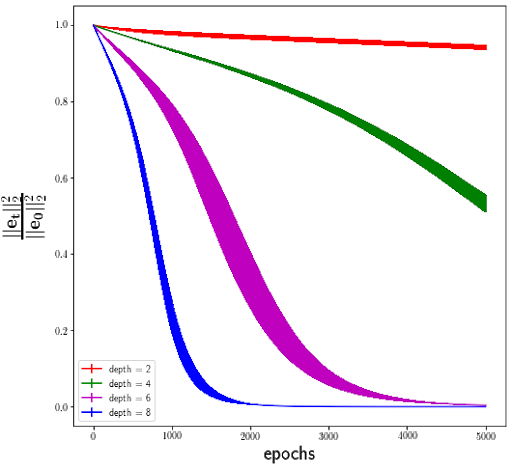
\includegraphics[scale=0.4]{figs/dgn-frg-conv-w100.png}
&
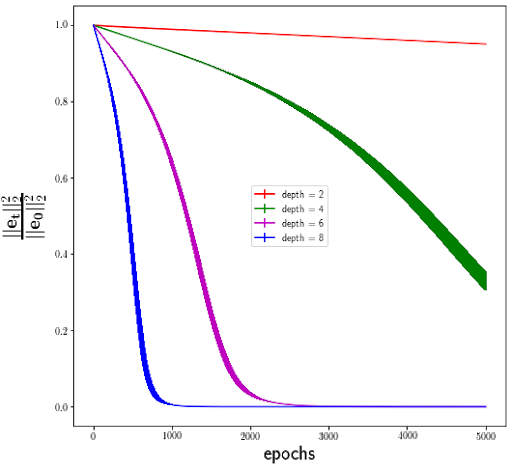
\includegraphics[scale=0.4]{figs/dgn-frg-conv-w500.png}
\end{tabular}
}
\caption{Show the rate of convergence with respect to depth for $w=100$ (left) and $w=500$ (right).}
\end{figure}

\subsection{Effect of Depth on GaLU and ReLU Networks}
We now look at $\N(\Tg_{\dagger}, \infty;\Tw_t)$ networks the gating is dictated by $\Tg_{\dagger}$, i.e., $\Tg_t=\Tg_0,\forall t\geq 0$. Also note that as per Assumption~\ref{assmp:mainone}, we have $\Tg_0$ to be statistically independent of $\Tw_0$, which are sampled as per Assumption~\ref{assmp:maintwo}. Due to the symmetric nature of the weights, we can expect roughly half the number of gates to be \emph{on}, and it follows that $\mathbf{E}_{\Tg_0}\left[ \mu^{s,s}\right]=d(p\sigma^2)^{d-1}$ with $p=\frac12$. However, for two distinct input examples $s$ and $s'$, $\frac{\mathbf{E}_{\Tg_0}\left[ \mu^{s,s'}\right]}{\mathbf{E}_{\Tg_0}\left[ \mu^{s,s}\right]}\leq p^{d-1}$ might not hold with $p=\frac12$. That said, since not all active paths overlap for $s$ and $s'$, one can still expect $\frac{\mathbf{E}_{\Tg_0}\left[ \mu^{s,s'}\right]}{\mathbf{E}_{\Tg_0}\left[ \mu^{s,s}\right]}\leq \gamma^{d-1}$, for some $\gamma\in (0,1)$.

\textbf{Experiment:} We consider dataset $(x_s,y_s)_{s=1}^{n}\in \R^2\times \R$, where, $n=200$ and $x_s\stackrel{iid}\sim unif(\left[-1,1\right]^2)$ and $y_s\stackrel{iid}\sim unif([-1,1])$. The results are shown in \Cref{fig:galu-d}. The trend is similar to DGN-FRG case, in that, both e.c.d.f as well as convergence get better with increasing depth. We also observe that GaLU, i.e., $\N(\Tg_{\dagger},\infty;\Tw_t)$ networks optimise better than $\N(\Theta_t,\infty;\Theta_t)$ networks, it is also true that the e.c.d.f for the case of GaLU is better than that of ReLU. This can be attributed to the fact that, in ReLU network the dot product of two different active paths is not zero and hence the Gram matrix entries fall back to the expression in \Cref{rm:basicgram}.
\FloatBarrier
\begin{figure}[h]
\resizebox{\columnwidth}{!}{
\begin{tabular}{cc}
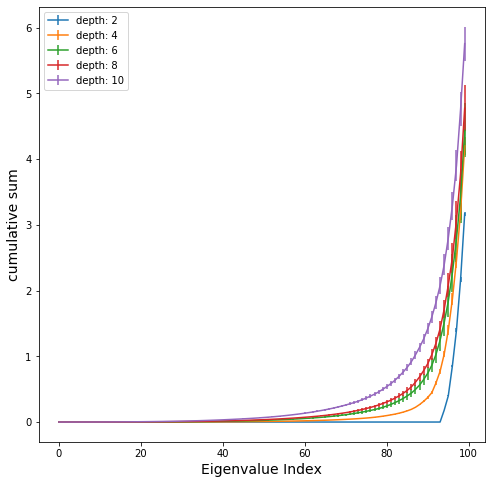
\includegraphics[scale=0.4]{figs/galu-ecdf-d.png}
&
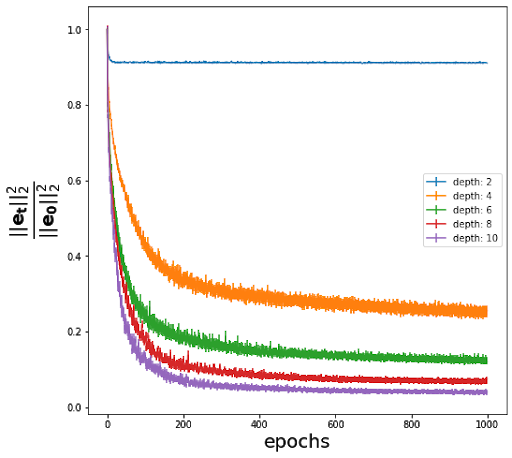
\includegraphics[scale=0.4]{figs/galu-conv-d.png}
\end{tabular}
}
\caption{Shows e.c.d.f (left) and convergence rates for various depth in GaLU networks.}
\label{fig:galu-d}
\end{figure}

%\subsection{Effect of Depth on ReLU and ReLU vs GaLU}

\FloatBarrier
\begin{figure}[h]
\resizebox{\columnwidth}{!}{
\begin{tabular}{cc}
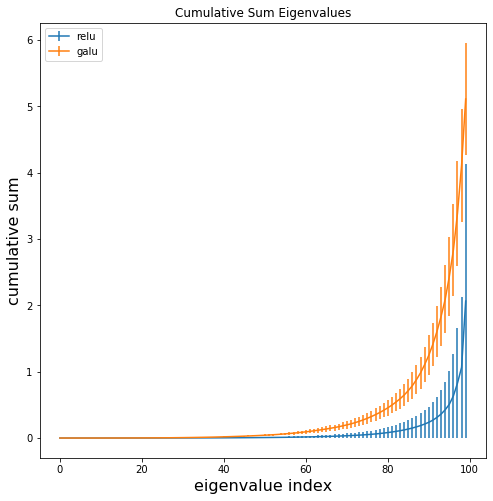
\includegraphics[scale=0.4]{figs/galu-relu-ecdf.png}
&
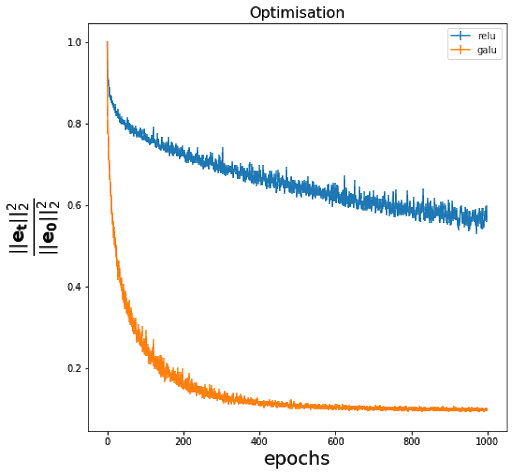
\includegraphics[scale=0.4]{figs/galu-relu-opt.png}
\end{tabular}
}
\end{figure}

